\documentclass{ximera}
\handouttrue

% vier voorkeuren die je meteen zelf kan instellen:
\def\uitbr{0} % waarde 1 als je Uitbreiding in de marge wilt, 0 als je dat niet wilt 
\def\wsg{0} % waarde 1 als je verwijzingen naar Wiskunde Samen gevat² in de marge wilt, 0 als je dat niet wilt
\def\rectoverso{0} % waarde 1 als je het PDF-bestand recto-verso wilt laten afdrukken, 0 als je het recto wilt
\def\voetn{1} % waarde 1 als je de voetnoten wilt, 0 als je dat niet wilt 

% marges:
\usepackage[paper=a4paper,margin=3.4cm,marginparwidth=2cm]{geometry}

% packages algemeen:
\pdfOnly{
\usepackage[english,dutch]{babel}
}
\usepackage{amsfonts}
\usepackage{amsmath} %  o.a. \eqref en \text, omgeving equation*
\usepackage{amssymb} % o.a. \nmid
\usepackage{amsthm} % o.a. omgeving proof
\usepackage{graphicx} % o.a. figuren
\usepackage{xcolor} % \color
\usepackage[disable]{todonotes} % \todo 
\usepackage{comment} % omgeving comment
\usepackage{xcolor} % kleuren 
\usepackage[skip=7pt plus1pt, indent=0pt]{parskip} % skip = verticale ruimte tussen twee alinea's, indent = insprong bij nieuwe alinea
\usepackage{multicol} % kolommen
\usepackage{xfrac} % breuken

\usepackage{siunitx} % SI eenheden
\usepackage{eso-pic} % achtergrond voorpagina
\usepackage{tabularx} % kolommen voor rekenmachine
\usepackage{rotating} % voor omgeving turn

% voor figuren met PSTricks:
\usepackage{pstricks} 
\usepackage{pstricks-add}
\usepackage{pst-plot}
\usepackage{pst-node}
\usepackage{pst-coil}
\usepackage{auto-pst-pdf}

% voor figuren met TikZ:
\usepackage{tikz} 
\usepackage{tkz-euclide} 
\usepackage{pgfplots} 
\usetikzlibrary{calc,intersections,through,backgrounds,patterns} 
\pgfplotsset{compat=newest}
\usepgfplotslibrary{fillbetween,colormaps}
\usepackage{import}
\usepackage{tikz-3dplot}

% zelfde parskip in minipage:
\makeatletter
\setlength{\parskip}{\medskipamount}
\newcommand{\@minipagerestore}{\setlength{\parskip}{\medskipamount}}
\makeatother

% voor veranderen van de naam Bibliografie naar Referentielijst:
\pdfOnly{
\addto\captionsdutch{\renewcommand{\bibname}{Referentielijst}}

% voor trefwoordenlijst:
\usepackage{imakeidx}
\makeindex[title=Trefwoordenlijst,program=makeindex,options=-s index.tex,columns=2,intoc=true]
}
% voor nummeren van vergelijkingen:
%WIM%\numberwithin{equation}{chapter} % als je dit desactiveert dan worden vergelijkingen in bijvoorbeeld hoofdstuk 3 genummerd als (1), (2) etc. in plaats van (3.1), (3.2) etc.

% voor hyperlinks en bladwijzers in PDF-bestand:
%WIM%\usepackage[bookmarksopen,bookmarksopenlevel=0,hypertexnames=false,pdfa,bookmarksnumbered]{hyperref} 
%WIM%\usepackage{bookmark} 

% voor hyperlinks: 
\hypersetup{pdfborder={0 0 0}, pdfstartpage=1,linkbordercolor={1 0 0}}%pdfborder={0 0 0} is geen rand rond hyperlinks, pdfborder={1 1 1} wel

% korter commando voor displaystyle, om bijvoorbeeld breuken groter te drukken in doorlopende tekst: 
\newcommand{\D}{\displaystyle}

% (veel)gebruikte verzamelingen:
\newcommand\NN{\mathbb{N}} % verzameling van de natuurlijke getallen
\newcommand\QQ{\mathbb{Q}} % verzameling van de rationale getallen
\newcommand\RR{\mathbb{R}} % verzameling van de re\"ele getallen
\newcommand\ZZ{\mathbb{Z}} % verzameling van de gehele getallen

% (veel)gebruikte operatoren:
\def\co{\operatorname{co}} % coördinaat van een punt
\def\ggd{\operatorname{ggd}} % positieve grootste gemene deler van twee gehele getallen niet beide nul
\def\gr{\operatorname{gr}} % graad van een veelterm

% voor kleur grafieken (donkergroen):
\definecolor{graf}{RGB}{0,100,0} 

% voor lijsten: 
% \usepackage{enumerate}
%WIM%\usepackage[shortlabels]{enumitem} 
\setlist{topsep=0em, itemsep=-0.15em}

% voor small bullet:
\newcommand\sbullet[1][.5]{\mathbin{\vcenter{\hbox{\scalebox{#1}{$\bullet$}}}}}

% voor meer verticale ruimte tussen vergelijkingen in align
\addtolength{\jot}{0.1cm}

% voor meervoudige voetnoten:
\usepackage{fnpct}

% voor het onderdrukken van voetnoten als optie:
\usepackage{letltxmacro}
\LetLtxMacro\Oldfootnote\footnote
\newcommand{\EnableFootNotes}{%
  \LetLtxMacro\footnote\Oldfootnote%
}
\newcommand{\DisableFootNotes}{%
  \renewcommand{\footnote}[2][]{\relax}
}

% voor verticale lijn in de marge (uitbreiding):
\usepackage[framemethod=default]{mdframed}
\usepackage{marginnote}
\reversemarginpar
\ifthenelse{\uitbr < 1}{\definecolor{rood}{RGB}{255,255,255}}{\definecolor{rood}{RGB}{254,64,64}} %HEX: #fe4040
\mdfdefinestyle{uitbreiding}{%
    topline=false,
    rightline=false,
    bottomline=false,
    leftline=true,
    linecolor=rood,
    linewidth=5pt,
    rightmargin=0pt,
    skipabove=10pt,% ipv 3
    skipbelow=0pt,
    leftmargin=-25pt,
    innerleftmargin=20pt,
    innerrightmargin=0pt,
    innertopmargin=0pt,
    innerbottommargin=0pt%,
%	needspace=30pt %minimumhoogte vooraleer lijn wordt gesplitst
    }
\newenvironment{Uitbreiding}{
    \marginpar{
        \center
		\vspace{0.1cm}
		\vspace{7pt}
		\rotatebox{90}{\color{rood}\Large \bf Uitbreiding}
	}
    \begin{mdframed}[style=uitbreiding]
    }{\vspace{-0.05cm}
    \end{mdframed}
}


% omgevingen voor lemma, definitie, voorbeeld etc.:
\newtheoremstyle{mystyle}
    {0em} % Space above
    {0em} % Space below
    {\itshape} % Body font
    {} % Indent amount
    {\bfseries} % Theorem head font
    {.} % Punctuation after theorem head
    {.5em} % Space after theorem head
    {} % Theorem head spec (can be left empty, meaning `normal')
\theoremstyle{mystyle}
%WIM%\newtheorem{lemma}{Lemma}[chapter] % als je [chapter] desactiveert dan Voorbeeld 3 in plaats van Voorbeeld 5.3, als je [chapter] vervangt door [section] dan Voorbeeld 5.2.3 in plaats van Voorbeeld 5.3 
%\theoremstyle{definition} % als je dit activeert dan is wat in de omgeving staat niet cursief gedrukt
\newtheorem{oefening}[lemma]{Oefening}
\newtheorem{definitie}[lemma]{Definitie} 
\newtheorem{voorbeeld}[lemma]{Voorbeeld}
\newtheorem{eigenschap}[lemma]{Eigenschap} 
\newtheorem{stelling}[lemma]{Stelling} 
\newtheorem{gevolg}[lemma]{Gevolg} 
\newtheorem{afspraak}[lemma]{Afspraak} 
\newtheorem{werkwijze}[lemma]{Werkwijze}

% omgeving proof, aangepaste ruimte: 
\makeatletter
\renewenvironment{proof}[1][\proofname]{\par
  \vspace{-\topsep}% remove the space after the theorem
  \pushQED{\qed}%
  \normalfont
  \topsep0pt \partopsep0pt % no space before
  \trivlist
  \item[\hskip\labelsep
        \itshape
    #1\@addpunct{.}]\ignorespaces
}{%
  \popQED\endtrivlist\@endpefalse
  \addvspace{0pt plus 0pt} % no space after
}
\makeatother

% kaderstijlen uit SOHO Wiskunde Plantyn:
\colorlet{steunkleur}{black}
\colorlet{steunkleurlicht}{steunkleur!30!white}
\colorlet{steunkleurkader}{steunkleur!7!white}
\colorlet{steunkleurkaderlicht}{steunkleur!2!white}

\mdfdefinestyle{kaderstijl_vol_licht}
{skipabove=6pt, 
skipbelow=6pt, 
backgroundcolor=steunkleurkader,
linecolor=steunkleurlicht,
linewidth = 0.4pt, 
topline=true,
bottomline=true, 
rightline=true,
innerleftmargin=5pt,
innerrightmargin=5pt,
innertopmargin=5pt,
leftmargin=0cm,
rightmargin=0cm,
innerbottommargin=5pt,
needspace=30pt % minimumhoogte voor splitsen kader
}
\surroundwithmdframed[style=kaderstijl_vol_licht]{definitie}
\surroundwithmdframed[style=kaderstijl_vol_licht]{stelling}
\surroundwithmdframed[style=kaderstijl_vol_licht]{lemma}
\surroundwithmdframed[style=kaderstijl_vol_licht]{eigenschap}
\surroundwithmdframed[style=kaderstijl_vol_licht]{gevolg}

% voor omgevingen voor oefening en antwoord:
\newenvironment{Oefening}{%
    \begin{enumerate}[ 
    series=Oef,
    resume=Oef,
    leftmargin=1.78em,
    label={\bfseries\arabic*.},
    ref=\arabic*
    ]
    \item %
    }{%
    \end{enumerate}
}
\newenvironment{Antwoord}{%
    \begin{enumerate}[%
    series=Antw,
    resume=Antw,
    leftmargin=1.78em,
    label={\bfseries\arabic*.},
    ref=\arabic*
    ]
    \item %
    }{%
    \end{enumerate}
}

% als de omgeving Uitbreiding start met een kaderomgeving (definitie, stelling, eigenschap, lemma of gevolg) dan moet wat extra verticale ruimte voorzien worden, met het commando \uitbreidingstartmetkader:
\def\uitbreidingstartmetkader{\mbox{}\vspace{-0.205cm}}

% % voor schema van de staartdeling:
% \usepackage{stackengine}
% \setstackgap{S}{5pt}
% \stackMath\def\stackalignment{r}
% \newcommand{\myRule}[3][white]{\textcolor{#1}{\rule{#2}{#3}}}
% \let\ph\phantom % enkel voor tekst
% \newcommand{\mph}[1]{% enkel voor math mode
%     \mathcolor{white}{#1}%
% }
% \def\staartmin{\rule{0.25cm}{0.1mm}\myRule{0.3cm}{0.1mm}}
% \def\staartphmin{\myRule{0.25cm}{0.1mm}\myRule{0.3cm}{0.1mm}}
% \newcommand{\staartstreep}[1]{\rule{\widthof{$#1$}}{0.1mm}}
% \newcommand{\staartphstreep}[1]{\myRule{\widthof{$#1$}}{0.1mm}}

% voor kolommen met schema van Horner:
\newcommand{\kolbreed}{1.0cm}
\newcolumntype{H}{>{\centering\arraybackslash$} p{\kolbreed} <{$}}

% voor nieuw commando utikzdashed: onderlijn (zoals underline) maar dan met stippellijn:
\tikzset{
    cheating dash/.code args={on #1 off #2 ends #3}{%
        \csname tikz@addoption\endcsname{%
            \pgfgetpath\currentpath%
            \pgfprocessround{\currentpath}{\currentpath}%
            \csname pgf@decorate@parsesoftpath\endcsname{\currentpath}{\currentpath}%
            \pgfmathparse{max(#1-#3,0)}\let\dashphase=\pgfmathresult%
            \pgfmathparse{\csname pgf@decorate@totalpathlength\endcsname-#1+2*\dashphase}\let\rest=\pgfmathresult%
            \pgfmathparse{#1+#2}\let\onoff=\pgfmathresult%
            \pgfmathparse{max(floor(\rest/\onoff), 1)}\let\nfullonoff=\pgfmathresult%
            \pgfmathparse{max((\rest-\onoff*\nfullonoff)/\nfullonoff+#2, #2)}\let\offexpand=\pgfmathresult%
            \pgfsetdash{{#1}{\offexpand}}{\dashphase pt}}%
    },
    cheating dash per segment/.style args={on #1 off #2 ends #3}{
        /utils/exec=\csname tikz@options\endcsname,%
        decoration={show path construction,
            lineto code={\draw [cheating dash=on #1 off #2 ends #3] (\tikzinputsegmentfirst) -- (\tikzinputsegmentlast);},
            curveto code={\draw [cheating dash=on #1 off #2 ends #3] (\tikzinputsegmentfirst) .. controls (\tikzinputsegmentsupporta) and (\tikzinputsegmentsupportb) .. (\tikzinputsegmentlast);},
            closepath code={\draw [cheating dash=on #1 off #2 ends #3] (\tikzinputsegmentfirst) -- (\tikzinputsegmentlast);}
        },
        decorate,
    },
}
\newcommand{\utikzdash}[1]{%
    \tikz[baseline=(todotted.base)]{
        \node[inner sep=0pt,outer sep=1.5pt] (todotted) {#1};
        \draw[cheating dash per segment=on 2pt off 2pt ends 2pt, line width=0.4pt] (todotted.south west) -- (todotted.south east);
    }%
}%

\providecommand{\xmemph}[1]{\textit{#1}}

% voor nieuw commando underdashed: onderlijn met stippellijnen en ook het woord cursief zetten:
\newcommand{\underdashed}[1]{%
    {\em\utikzdash{\!#1\!}}%
}

% voor icoon TI-84 Plus met verwijzing naar filmpje:
\newcommand{\grmlink}{\raisebox{0cm}{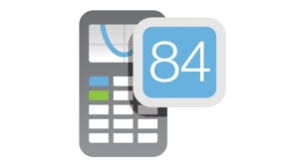
\includegraphics[width=1cm]{TI84Plus-icoon}}}
\newcommand{\grmref}[1]{%
	\reversemarginpar%
	\marginpar{
		\vspace{-0.4cm}%
		\htmladdnormallink{\grmlink}{#1}
	}	
}

% GRM knoppen:
\newcommand{\GRM}[1]{\fbox{\rule[0mm]{0cm}{0.215cm}\textup{\texttt{#1}}}}
\newcommand{\wedgetext}{{\raisebox{0.02cm}{\begin{turn}{90}>\end{turn}}}}
\newcommand{\veetext}{\raisebox{0.2cm}{\begin{turn}{-90}>\end{turn}}}

% voor kolommen met GRM screens:
\newlength{\widthallscreens}
\newlength{\widthscreens}
\newlength{\spaceleftscreen}
\newlength{\spacerightscreen}
\newlength{\spacebetweenscreens}

\newcommand{\setscreens}{
	\setlength{\spaceleftscreen}{2pt}
	\setlength{\spacerightscreen}{2pt}
	\setlength{\spacebetweenscreens}{8pt}
	\addtolength{\linewidth}{-28pt} % 3*8pt tussen vier screens en 2 pt links en 2 pt rechts
	\setlength{\widthallscreens}{\linewidth}
	\setlength{\widthscreens}{0.25\widthallscreens}
	\addtolength{\linewidth}{28pt}
	\newcolumntype{G}{p{\widthscreens}}
	\newcolumntype{s}{p{\spacebetweenscreens}}
	\newcolumntype{L}{p{\spaceleftscreen}}
	\newcolumntype{R}{p{\spacerightscreen}}
	\setlength{\tabcolsep}{0pt}
}

% voor icoon met verwijzing naar Wiskunde Samen gevat² in de marge:
% \newcommand{\wsglink}{\raisebox{0cm}{\includegraphics[width=1cm]{wsglogo}}}
\newcommand{\wsglink}{\raisebox{0cm}{LOGO}}
\newcommand{\htmladdnormallink}[2]{\href{#2}{#1}}
\newcounter{pagnrwsg}
\newcommand{\wsgref}[3]{% 
    % #1 woord dat onderstippeld wordt
    % #2 pagina van Wiskunde Samen gevat² waar je op terecht komt als je op de link klikt  
    % #3 afgedrukt op het logo van Wiskunde Samen gevat² in de marge: één of meerdere paginanummers
    \ifthenelse{\wsg < 1}{#1}{%
        \underdashed{#1}%
        {\setcounter{pagnrwsg}{#2}}%
        {\addtocounter{pagnrwsg}{14}}%
        \reversemarginpar%
        \marginpar{\vspace{-0.6cm}%
           \htmladdnormallink{\wsglink}{https://online.fliphtml5.com/sanky/laea/\#p=\arabic{pagnrwsg}}%
            \raisebox{0.41cm}[0cm][0cm]{%
                \hspace{-1.5cm}\makebox[2cm][c]{\colorbox{white}{\texttt{\footnotesize{#3}}}}%
            }%
        }%
    }%
}

% voor invoegen blanco pagina bij de optie recto-verso:
\def\blancobijrectoverso{
	\ifthenelse{\rectoverso < 1}{\clearpage}{
	\clearpage
	\thispagestyle{empty}
	\mbox{}
	\clearpage
	}
}

% aantal pagina's van het bestand:
\ifthenelse{\rectoverso < 1}{\def\totpag{57}}{\def\totpag{66}}

% documenteigenschappen:
% \usepackage{hyperxmp}
% \hypersetup{
% pdftitle={Open Source Wiskunde Aan zet: Veeltermen}, 
% pdfnumpages={\totpag},
% pdfauthor={Koen De Naeghel},
% pdflang={nl},
% pdfkeywords={wiskunde, open source, wiskunde aan zet, veeltermen, secundair onderwijs, tweede graad, doorstroomfinaliteit},
% pdfsubject={Veeltermen},
% pdfcopyright={\unichar{"24B8} 2024 Koen De Naeghel},
% pdfdate={17 december 2024},
% pdfapart=1,
% pdfstartview=}

% voor het benoemen van titel, auteur en datum:
% \title{Veeltermen}
% \author{Auteur: Koen De Naeghel}
% \date{\today}

\newcommand\BackgroundPic{
    \put(-260,-125){
    \parbox[b][\paperheight]{\paperwidth}{%
    \vfill
    \centering
    
\includegraphics[height=\paperwidth, keepaspectratio]{WaZlogo}%
    \vfill
}}}

\addPrintStyle{..}
\begin{document}
	\author{Wim Obbels}
	\xmtitle{Complexe getallen (algebraisch)}{}
	% \xmtitle{Complexe getallen (algebraïsch)}{}
	\label{xim:cmplx_definitie_algebraisch}
    
Met een nieuwe symbool $i$  worden er nieuwe getallen ingevoerd. 
Er ontstaan combinaties als $2i$ en $i+1$, die we \textbf{complexe getallen} noemen, niet omdat ze ingewikkeld zijn, maar omdat ze zijn \textit{samengesteld}  uit reële getallen en het nieuwe symbook $i$.


\begin{definition}[Complex getal]\label{def:complex_getal}\label{def:reeel_deel}\label{def:imaginair_deel}\nl
	
    Een \textbf{complex getal} is een uitdrukking van de vorm \(a+bi\), met \(a,b \in \R\).
    \\
    Het symbool \(i\) waarvoor \( \important{i^2=-1}\) noemen we de \textbf{imaginaire eenheid}.
    
De \textbf{verzameling complexe getallen} noteren we met \(\important{\C=\{a+bi \;|\; a,b\in\R;\; i^2=-1\}} \).

Voor een complex getal $z=a+bi$ noemen we: \\
\begin{tabular}{@{\quad}l@{ }ll}    
    & $a=\Re(a+bi)=\Re(z)$ het \textbf{reëel deel}  \\
    & $b=\Im(a+bi)=\Im(z)$ het \textbf{imaginair deel}.
\end{tabular}

\begin{tabular}{@{}l@{ }ll}    
    Als $\Im(z) = b=0$, dan is $z=a$ & een \textbf{(zuiver) re\"eel getal}  \\%& en $\R$ is dus een deelverzameling van $\C$,\\
    Als $\Re(z) = a=0$, dan is $z=bi$ & een \textbf{(zuiver) imaginair getal}.
\end{tabular}
    
    
Twee complexe getallen zijn \textbf{gelijk} indien ze  dezelfde reële en imaginaire delen hebben:
\vspace{-0.35cm}
\begin{center}
    \begin{tabular}{rcl}
        \(z = w\) &\(\iff\)& \(\Re(z)=\Re(w) \Ten \Im(z)=\Im(w)\) \\    
        \(a+bi = c + di \)  &\(\iff\)& \(a = c \Ten b = d \)\\   
    \end{tabular}
\end{center}

\end{definition}

%\begin{expandable}{remark}{Notatie}
    Complexe getallen worden dikwijls met de letters \(z\) of \(w\) genoteerd, net zoals we voor een natuurlijk getal \(n\) gebruiken of voor functies \(f, g \) en \(h\).
%\end{expandable}

\begin{expandable}{remark}{Gelijkheid van complexe getallen}
    Het kan overbodig lijken om te vermelden wanneer twee complexe getallen \(z = a+bi\) en \(w = c+di\) aan elkaar gelijk zijn. Merk op dat een gelijkaardige regel voor breuken \textit{niet} geldt: als $\frac{a}{b} = \frac{c}{d}$ gelijk zijn hoeft niet te gelden dat \(a = c\) en \(b = d\). De breuken $\frac{1}{2}$ en $\frac{3}{6}$ zijn immers gelijk, maar hun tellers en noemers toch zijn verschillend. 
\end{expandable}

% \begin{example}{Enkele complexe getallen met hun imaginair en reëel deel.}
%     \[
%     \begin{array}{c@{\quad}|@{\quad}r@{\quad}r}
%         z & \Re(z) & \Im(z) \\\hline
%         2+3i & 2 & \answer{3} 
%         \\
%         5-6i &\answer{5} & \answer{-6} 
%     \end{array}
%     \qquad
%     \begin{array}{c@{\quad}|@{\quad}r@{\quad}r}
%         z & \Re(z) & \Im(z) \\\hline
%         42 & 42 & 0 
%         \\
%         42i & 0 & 42
%     \end{array}
%     \qquad
%     \begin{array}{c@{\quad}|@{\quad}r@{\quad}r}
%         z & \Re(z) & \Im(z) \\\hline
%         1+i\sqrt{2} & 1 & \sqrt{2}
%         \\
%         1+\pi & 1+\pi & 0 
%         \\
%     \end{array}
%     \]
% De getallen $42$ en $1+\pi$ zijn zuiver reële getallen. Het getal $42i$ is een zuiver imaginair getal. 
% % \\
% \end{example}

\begin{example} Volgende uitdrukkingen zijn allemaal complexe getallen:
    $$
    \def\arraystretch{1.5}
    \begin{array}{c|rr c lll}
        z & \Re(z) & \Im(z) \\\hline
        2+3i & 2 & \answer{3} 
        \\
        5-6i &\answer{5} & \answer{-6} 
        \\
        1+i\sqrt{2} & 1 & \sqrt{2}
        \\
        \dfrac{1-i\sqrt{5}}{2}  & \dfrac{1}{2} & -\dfrac{\sqrt{5}}{2}
        \\
    \end{array}
    \qquad\qquad
    \begin{array}{c|rr c lll}
        z & \Re(z) & \Im(z) \\\hline
        1+\pi & 1+\pi & 0
        \\
        42 & \answer{42} & 0
        \\
        42i & \answer{0} & \answer{42} 
        \\
        5i + 7 & \answer{7} & \answer{5} 
        \\
        2+ 5i + \pi & \answer{2+\pi} & \answer{5} 
        \\
    \end{array}
    $$
    De getallen $42$ en $1+\pi$ zijn zuiver reële getallen, $42i$ is een zuiver imaginair getal. 
    \\
    \end{example}


    \begin{exercise} Geef telkens het reëel en het imaginair deel van de volgende complexe getallen.
        %\begin{xmmulticols}
        \renewcommand{\xmFixFormatLength}{10ex}
        \renewcommand{\xmFixFormatPosition}{c}
        \begin{question}
            \xmFixFormat{\(8+3i\)} heeft reëel deel $\answer{8}$ en imaginair deel $\answer{3}$. 
            \begin{oplossing} 
                Het reëel en imaginair deel van een complex getal vind je door het getal te schrijven in de vorm $a+bi$,
                en dan is 
                \(\Re(a+bi) = a\) en \(\Im(a+bi) = b\).
    
                Hier wordt dat dus \(\Re(8+3i) = 8\) en \(\Im(8+3i) = 3\).
            \end{oplossing}
        \end{question}
        
        \begin{question}
            \xmFixFormat{\(\sqrt{2} - \sqrt{2}i\)} heeft reëel deel $\answer{\sqrt{2}}$ en imaginair deel $\answer{-\sqrt{2}}$. 
        \end{question}
        \begin{question}
            \xmFixFormat{\(7i\)} heeft reëel deel $\answer{0}$ en imaginair deel $\answer{7}$. 
        \end{question}
        \begin{question}
            \xmFixFormat{\(5\)} heeft reëel deel $\answer{5}$ en imaginair deel $\answer{0}$. 
        \end{question}
        \begin{question}
            \xmFixFormat{\(5i-4\)} heeft reëel deel $\answer{-4}$ en imaginair deel $\answer{5}$. 
        \end{question}
        \begin{question}
            \xmFixFormat{\(\frac{1+2i}{3}\)} heeft reëel deel $\answer{\frac{1}{3}}$ en imaginair deel $\answer{\frac{2}{3}}$. 
        \end{question}
        \begin{question}
            \xmFixFormat{\(i\)} heeft reëel deel $\answer{0}$ en imaginair deel $\answer{1}$. 
        \end{question}
        \begin{question}
            \xmFixFormat{\(\frac{9+3i}{3}\)} heeft reëel deel $\answer{3}$ en imaginair deel $\answer{1}$. 
        \end{question}
        \begin{question}
            \xmFixFormat{\(\pi + i + e\)} heeft reëel deel $\answer{\pi+e}$ en imaginair deel $\answer{1}$.
        \end{question}
        \begin{question}
            \xmFixFormat{\(0\)} heeft reëel deel $\answer{0}$ en imaginair deel $\answer{0}$.
        \end{question}
        \begin{question}
            \xmFixFormat{\(\frac{\sqrt{5} + \sqrt{5}i }{\sqrt{5}}\)} heeft reëel deel $\answer{1}$ en imaginair deel $\answer{1}$. 
        \end{question}
        
        %\end{xmmulticols}
        
    \end{exercise}
        
    \begin{exercise} Schrijf zo eenvoudig mogelijk, door gebruik te maken van de gelijkheid $i^2=-1$.
        \renewcommand{\xmFixFormatLength}{3ex}
        \renewcommand{\xmFixFormatPosition}{r}
    
        \begin{xmmulticols}[5]
        \begin{question} \xmFixFormat{\( i^2\)}     = $\answer{-1}$	\end{question}
        \begin{question} \xmFixFormat{\( i^5\)}     = $\answer{i}$	\end{question}
        \begin{question} \xmFixFormat{\(-i^3\)}     = $\answer{i}$	\end{question}
        \begin{question} \xmFixFormat{\( i^4\)}     = $\answer{-1}$	\end{question}
        \begin{question} \xmFixFormat{\(-i^4\)}     = $\answer{-1}$	\end{question}
        \begin{question} \xmFixFormat{\(i^{10}\)}   = $\answer{-1}$	\end{question}
        \begin{question} \xmFixFormat{\(i^{11}\)}   = $\answer{-i}$	\end{question}
        \begin{question} \xmFixFormat{\(i^{12}\)}   = $\answer{1}$	\end{question}
        \begin{question} \xmFixFormat{\(-i^2\)}     = $\answer{1}$	\end{question}
        \begin{question} \xmFixFormat{\(i^{2028}\)} = $\answer{1}$	\end{question}
        \end{xmmulticols}
    \end{exercise}
    

\end{document}

